%%%%%%%%%%%%%%%%%%%%%%%%%%%%%%%%%%%%%%%%%%%%%%%%%
%       Macroscopic analysis of load curve      %
%   Antoine                                     %
%%%%%%%%%%%%%%%%%%%%%%%%%%%%%%%%%%%%%%%%%%%%%%%%%
\subsection{Macroscopic Analysis of a Load Curve}
A fast algorithm is needed and that can be called at any moment to detect a device. It is based on a study of the load curve. In case the results of this approach are doubtful, the microscopic algorithms are used.

The following approach comes from the work achieved by Mr. El Guedri \cite{research1}. The macroscopic algorithms are based on the differentiate function, which helps detect a jump in the load curve. Indeed the difference between two points of a jump is directly the consumption of the device, as shown in \ref{fig1} where the grouped squares are a heater use.


\begin{figure}[h]
 \begin{center}
   \subfloat[Example of a real load curve]{
   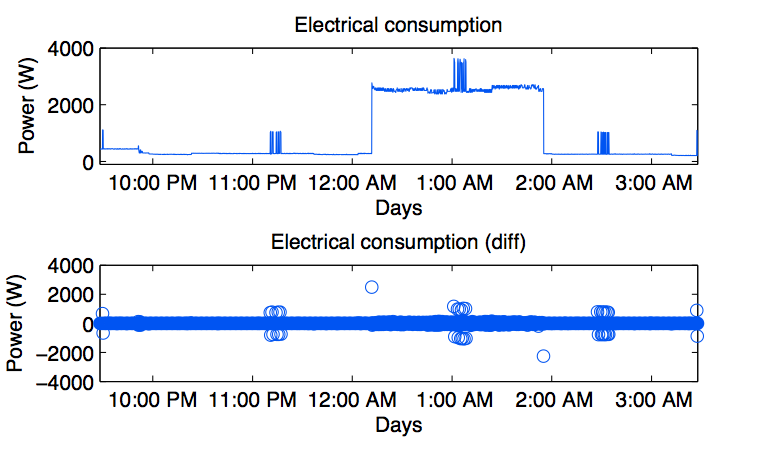
\includegraphics[width=0.45\textwidth]{figures/fig_antoine_5.png}
   \label{fig1}
   }
   \subfloat[Estimation of a heater consumption]{
   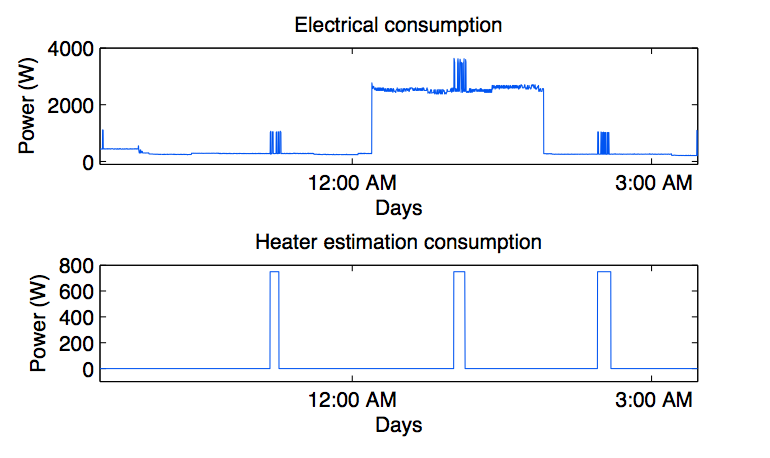
\includegraphics[width=0.45\textwidth]{figures/fig_antoine_6.png}
   \label{fig2}
   }
   \caption{Macroscopic Analysis}
   \label{fig-1-1-2}
 \end{center}
\end{figure}

Several steps of consumption were defined: $100$, $500$ and $750W$ which mean small consumption device (such as lights), medium consumption (oven) and heavy consumption (heater). The load curve reaching one of these values means the device is turning on, and reaching the same negative value means the device is turning off. With this basic approach some devices can be defined, but it is not possible to differentiate an unknown device consuming 500W from an oven for example.

Therefore, a second algorithm was developed that analyzes the signature load curve of each device. Every device has a specific and unique load curve when they turn on. If a data base were created with these signatures, they could be used to determine which device has just turned on. Spotting when the devices turn off is simple as it corresponds to negative values of the differentiate function.

An example will help make the description clearer. A heater power consumption load curve is basically a square repetition. This shape is due to the periodicity of the device. By detecting such a wave form in the load curve, then we can detect heater consumption and estimate the consumption of this device. These results are shown on the figure \ref{fig2}.


Non periodical devices are processed in the same way, such as a dishwasher or a washing machine. But at the moment, only the dishwasher has been implemented.

% Transition
% As the sampling frequency is quite low, to devices
